\documentclass[10pt]{article}

\usepackage[margin=2.5cm, includefoot, footskip=30pt]{geometry}

\usepackage{amssymb}
\usepackage{amsmath}
\usepackage{amsthm}
\usepackage{booktabs}
\usepackage{caption}
 \usepackage{epsfig}
\usepackage{graphicx}
\usepackage{hyperref}
\usepackage{psfrag}
\usepackage{subcaption}
\usepackage{ulem}
\usepackage{standalone}
\usepackage{tikz}
\usetikzlibrary{calc}
\usepackage{breakcites}
\usepackage{setspace}
\usepackage{lipsum}
\captionsetup{font=doublespacing}% Double-spaced float captions

\doublespacing% Double-spaced document text

\newcommand{\rd}{\mathrm{d}}
\newcommand{\be}{\begin{eqnarray}}
\newcommand{\ee}{\end{eqnarray}}
\usepackage{tabularx} % http://ctan.org/pkg/tabularx
\renewcommand{\arraystretch}{1.5} % tables have longer cells

\newtheorem{theorem}{Theorem}

\usepackage{lineno}

\title{An Evolutionary Game Theoretic Model of Rhino Horn Devaluation}
\author{Nikoleta E. Glynatsi, Vincent Knight, Tamsin E. Lee} %TODO Authors
\date{}

\begin{document}

\maketitle

\bigskip
\textbf{Keywords}: Evolutionary dynamics; Evolutionary stability; Game theory; \\
\indent Poachers' interactions; Rhinoceros; Wildlife

\bigskip

\textbf{Declaration of interest}: None.

\newpage
\linenumbers{}
\begin{abstract}

Rhino populations are at a critical level due to the demand for rhino horn and
the subsequent poaching. Wildlife managers attempt to secure rhinos with
approaches to devalue the horn, the most common of which is dehorning. Game theory
has been used to examine the interaction of poachers and wildlife managers where
a manager can either `dehorn' their rhinos or leave the horn attached and poachers
may behave `selectively' or `indiscriminately'. The approach described in this paper
builds on this previous
work and investigates the interactions between the poachers. We build an evolutionary
game theoretic model and determine which strategy is preferred by a poacher in various
different populations of poachers. The purpose of this work is to discover whether
conditions which encourage the poachers to behave selectively exist, that is,
they only kill those rhinos with full horns. Notwithstanding, the analytical
results prove that poachers will never adopt a selective strategy as long as
there is gain from a partial horn. Additionally, poachers behaving indiscriminately
is stable and robust. However, the model is adapted further to include a
disincentive factor, which may represent factors such as harsher punishment, or
lower demand for horn. With a disincentive, poachers can be encouraged to behave
selectively, but only when there are few devalued rhinos. This paper aims to
contribute to the necessary research required for informed discussion about the
lively debate on legalising rhino horn trade.

\end{abstract}

%=============================================
\section{Introduction}\label{section:introduction}

Rhino populations now persist largely in protected areas or on private land, and
require intensive protection~\cite{Ferreira2014} because the demand for rhino
horn continues to pose a serious threat~\cite{Amin2006}. The illegal trade in rhino
horn supports aggressive poaching syndicates and a black market~\cite{Nowell1992, Warchol2003}.
This lucrative market entices people to invest their time and energy to gain a
`windfall' in the form of a rhino horn, through the poaching of rhinos. In recent
years poaching has escalated to an unprecedented level resulting in concerns over
their future existence~\cite{Duan2013,Smith1993}. Several methods
include addressing the problem by reducing the demand in the market. In~\cite{Duan2013}
the authors suggest meeting the demand for rhino horn through a legal market by
farming the rhino horn from live rhinos. This controversial proposal is an active
conversation, with the actual quantity of horn that could be farmed being estimated
recently by \cite{Taylor2017}. Moreover, the debate is not limited to rhinos -
\cite{Harvey2017} considered ivory and stated that by enforcing a domestic ivory
trade ban we can reduce the market's demand.

Nonetheless, for wildlife managers law enforcement is often one of the main methods
to deter poachers.
In response, rhino conservation has seen increased  militarisation with `boots on the
ground' and `eyes in the sky'~\cite{duffy_st}. An alternative method is to
devalue the horn itself, one of the main  methods being the removal so that only
a stub is left. The first attempt at large-scale rhino dehorning as an anti-poaching
measure was in Damaraland, Namibia, in 1989~\cite{Milner1992}. Other methods
of devaluing the horn that have been suggested include
the insertion of poisons, dyes or GPS trackers~\cite{Gill2010,Smith1993}. However,
like dehorning, they cannot remove all the potential gain from an intact horn
(poison and dyes fade or GPS trackers can be removed and have been found to affect
only a small proportion of the horn).
In~\cite{Milner1992} they found the
optimum proportion to dehorn using mean horn length as a measure of the
proportion of rhinos dehorned. They showed, with realistic parameter values,
that the optimal strategy is to dehorn as many rhinos as possible.
A manager does not need to choose between law enforcement or devaluing, but
perhaps adopt a combination of the two; especially given that devaluing rhinos
comes at a cost to the manager, and the process comes with a risk to the rhinos.

A recent paper modelled the interaction between a rhino manager and poachers
using game theory~\cite{Lee}. The authors consider a working year of a single
rhino manager. A manager is assumed to have standard yearly resources which
can be allocated on devaluing a proportion of their rhinos or spent on security.
It is assumed that all rhinos initially have intact horns. Poachers may either only
kill rhinos with full horns, `selective poachers', or kill all rhinos they encounter,
`indiscriminate poachers'. This strategy may be preferred to avoid tracking a
devalued rhino again, and/or to gain the value from the partial horn. If all rhinos
are left by the rhino manager with their intact horns, it does not pay poachers to
be selective so they will chose to be indiscriminate since being selective incurs
an additional cost to discern the status of the rhino. Conversely, if all poachers are
selective, it pays rhino managers to invest in devaluing their rhinos.
Assuming poachers and managers will always behave so as to maximise their payoff,
there are two equilibriums: either all rhinos are devalued and all poachers are selective;
or all horns are intact and all poachers are indiscriminate. Essentially, either
the managers win and rhinos survive or the poachers win and rhinos are killed. The
paper~\cite{Lee} concludes that poachers will always choose to behave indiscriminately,
and thus the game settles to the bottom right quadrant, i.e., the poachers win.


In this manuscript, we explore the population dynamic effects associated to
the interactions described by~\cite{Lee}. More specifically, the interaction between
poachers.In a population full of indiscriminate poachers is there
a benefit to a single poacher becoming selective or vice versa? This notion
is explored here using evolutionary game theory~\cite{Smith}. The
game is not that of two players anymore (manager and poacher) but now the players
are an infinite population of poachers. This allows for the interaction between
poachers over multiple plays of the game to be explored with the rhino manager
being the one that creates the conditions of the population.

Note that poachers are, in practice finite, and each has individual factors that will
affect a poacher's behaviour. An infinite population model corresponds to either
an asymptotic generalisation or overall descriptive behaviour.

In evolutionary game theory, we assume infinite populations and in our
model this is represented by \(\chi=(x_1, x_2)\) with \(x_1\) being the proportion
of the population using a strategy of the first type and \(x_2\) of the second. We
assume there are utility functions \(u_1\) and \(u_2\) that map the population
to a fitness for each strategy, given by,

\[ u_1(\chi)  \text{ and } u_2(\chi).\]

In evolutionary game theory these utilities are used to dictate the evolution of
the population over time, according to the following differential equations,

\begin{eqnarray}
    \label{eqn:u_differential_eq}
    \left\{
    \begin{array}{cl}
    \dfrac{dx_1}{dt}=x_1(u_1(\chi)-\phi),
    \\
    \\
    \dfrac{dx_2}{dt}= x_2(u_2(\chi)-\phi),
    \end{array} \right.
\end{eqnarray}

In some settings these utilities are referred to as fitness and/or are mapped to
a further measure of fitness. This is not the case considered here (it is
assumed all evolutionary dynamics are considered by the utility measures).

where \(\phi\) is the average fitness of the whole population. Here, the overall
population is assumed to remain stable thus, \(x_1 + x_2 = 1 \) and

\begin{eqnarray}
    \dfrac{dx_1}{dt}  + \dfrac{dx_2}{dt} = 0 \Rightarrow x_1(u_1(\chi) - \phi)
     + x_2(u_2(\chi) - \phi)=0.
\end{eqnarray}

Recalling that \(x_1 + x_2 = 1\) the average fitness can be written as,

\begin{eqnarray}
\label{eqn:average_fitness}
    \phi=x_1u_1(\chi) + x_2u_2(\chi).
\end{eqnarray}

\noindent{} By substituting (\ref{eqn:average_fitness}) and \(x_2= 1 - x_1\)
in (\ref{eqn:u_differential_eq}),

\begin{eqnarray}
    \label{eqn:u_differential_simplified}
    \frac{dx_1}{dt}= x_1(1 - x_1)(u_1(\chi) - u_2(\chi)).
\end{eqnarray}

The equilibria of the differential equation (\ref{eqn:u_differential_simplified})
are given by, \(x_1=0\), \(x_1=1\), and \(0<x_1<1\) for \(u_1(\chi)=u_2(\chi)\).
These equilibria correspond to stability of the population: the differential
equation (\ref{eqn:u_differential_simplified}) no longer changes.

The notion of evolutionary stability can be checked only for these stable strategies.
For a stable strategy to be an Evolutionary Stable Strategy (ESS) it must remain
the best response even in a mutated population \(\chi_\epsilon\). A mutated population
is the post entry population
where a small proportion \(\epsilon > 0\) starts deviating and adopts a different strategy.
Fig.~\ref{fig:stable_ess_driagrams} illustrates two potential strategies: without
outside stimulation neither marble would move. In Fig.~\ref{fig:ess_diagram}
however the stability can be described as ``stronger": with a small nudge the marble
would return to its stable position. In Fig.~\ref{fig:stable_diagram} any non-zero
nudge would move the marble out of its equilibria.

\begin{figure}[!htbp]
\begin{center}
    \begin{subfigure}{0.35\textwidth}
    \includestandalone[width =\textwidth]{images/stable}
    \caption{\label{fig:stable_diagram} A diagram of a stable strategy which
    is not ESS.}
    \end{subfigure}
    \begin{subfigure}{0.35\textwidth}
    \includestandalone[width = \textwidth]{images/evolutionary_stability}
    \caption{\label{fig:ess_diagram}A diagram of a stable strategy which is ESS.}
    \end{subfigure}
        \caption{\label{fig:stable_ess_driagrams} Diagrams of stable strategies.}
\end{center}
\end{figure}

In Section~\ref{section:the_model}, we determine expressions
for \(u_1, u_2\) that correspond to a population of wild rhino poachers and we
explore the stability of the equilibria identified in~\cite{Lee}. The results
contained in this paper are proven analytically, and more specifically it is
shown that:

\begin{itemize}
    \item all poachers behaving selectively is trivially unstable,
    \item a mixed population where selective and indiscriminate poachers
          learn to coexist can not hold,
    \item all poachers adopting an indiscriminate strategy is an evolutionary
          stable strategy.
    % TODO Modify this after the new utility model is done
\end{itemize}

This implies that under almost all conditions, no matter what current proportion
of
of poachers are acting selectively, the population will eventually turn into a
population of only indiscriminate poachers.

%============================================================
\section{The Utility Model}\label{section:the_model}

As discussed briefly in Section~\ref{section:introduction}, a rhino poacher
can adopt two strategies, to either behave selectively
or indiscriminately. To calculate the utility for each strategy, the gain and cost
that poachers are exposed to must be taken into account. The poacher incurs a
loss from seeking a rhino, and the risk involved. The gain depends upon the value
of horn, the proportion of horn remaining after the manager has devalued the
rhino horn and the number of rhinos (devalued and not).

Let us first consider the gain to the poacher, where \(\theta\) is the amount of
horn taken. We assume rhino horn value is determined by weight only, a
reasonable assumption as rhino horn is sold in a grounded form~\cite{Saverhino}.
Clearly if the horn is intact, the amount of horn gained is \(\theta=1\) for both
the selective and the indiscriminate poacher.
If the rhino horn has been devalued, and the poacher is selective, the amount of
horn gained is \(\theta=0\) as the poacher does not kill. However, if the poacher
is behaving indiscriminately, the proportion of horn gained is \(\theta = \theta_r\)
(for some \(0<\theta_r<1\)). Therefore, the amount of horn gained in the
general case is

\begin{eqnarray}
    \label{eqn:theta}
    \theta(r, x) = x (1 - r) + (1 - x) ((\theta_r - 1) r + 1),
\end{eqnarray}
where \(r\) is the proportion of rhinos that have been devalued, and \(x\) is the
proportion of selective poachers and \(1-x\) is the proportion of indiscriminate
poachers. Note that since \(\theta_r, r, x  \in [0, 1]\), then
\(\theta(r, x) > 0\), that is, some horn will be taken. Standard supply and demand
arguments imply that the value
of rhino horn decreases as the quantity of horn available increases~\cite{mankiw2010}.
Thus at any given time the expected gain is

\begin{eqnarray}
    \label{eqn:individual_gain}
    H \theta(r, x)^{-\alpha},
\end{eqnarray}
where \(H\) is a scaling factor associated with the value of a full horn, and
\(\alpha \geq 0\) is a constant that determines the precise relationship between
the quantity and value of the horn.  Fig.~\ref{fig:GainCurve}, verifies that the
gain curve corresponds to a demand curve.

\begin{figure}[!htbp]
\centering
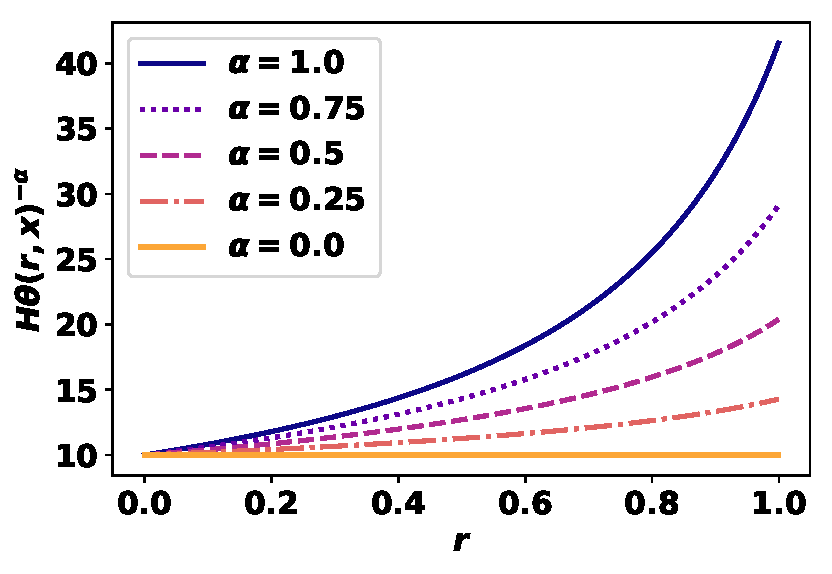
\includegraphics[width=0.4\textwidth]{images/gain_curve.pdf}
\caption{\label{fig:GainCurve} \(H \theta(r, x) ^{- \alpha}\) for values
\(H = 10, \theta_r = 0.3\) and \(x = 0.2.\)}
\end{figure}

An individual interacts with the population, denoted as \(\chi=(x,1-x)\) .
For simplicity, from herein the population \(\chi\) is referred to in terms
of the proportion of selective poachers only, \(x\).
Therefore, the gain for a poacher in the population \(x\) is either
% Beginning of some notation changes
\begin{eqnarray}
    \label{eqn:gain}
    \left\{
    \begin{array}{cl}
    \theta(r, 1) H \theta(r, x)^{-\alpha} & \mbox{ selective poacher}
    \\
    \theta(r, 0) H \theta(r, x)^{-\alpha} & \mbox{ indiscriminate poacher}
    \end{array} \right.
\end{eqnarray}
depending on the chosen strategy of the individual.

% TODO Re word this paragraph (specifically get rid of $\psi$) and just talk in
% terms of time spent in the park.
Secondly we consider the costs incurred by the poacher. Let us denote the number
of rhinos that will be considered at risk given \(r\) and \(x\) as \(\psi(r, x)\).
The rhinos \textbf{not} at risk are the devalued ones
that cross the paths of selective poachers. Thus the cost to seek a rhino depends
on \(r\) and \(x\) by,

\begin{eqnarray}
    \label{eqn:psi}
    \psi(r, x) = 1 - rx.
\end{eqnarray}


It is assumed that a given poacher will spend sufficient time in the park to
obtain the equivalent of a single Rhinoceros's horn. For selective poachers this
implies searching the park for a fully valued horn and for indiscriminate
poachers this implies either finding a fully valued horn or finding \(N_r\)
total Rhinoceroses where \(N_r = \lceil 1 / \theta_r \rceil\).

Figure~\ref{fig:random_walk} shows a random walk that any given poacher will
follow in the park. Both types of poacher will exit the park as soon as they
encounter a fully valued Rhino, which at every encounter is assumed to happen
with probability \(1 - r\). However, the indiscriminate poachers may also exit
the park if they encounter \(N_r\) devalued Rhinos in a row.
Each step on the random walk is assumed to last 1 time unit: during which a
Rhino is found.
To capture the fact that indiscriminate poachers will spend a different amount
of time with each Rhino the parameter \(t\) is introduced which corresponds to
the amount of time it takes to find and kill a Rhino (thus \(t\geq 1\)).

\begin{figure}[!htbp]
    \begin{center}
        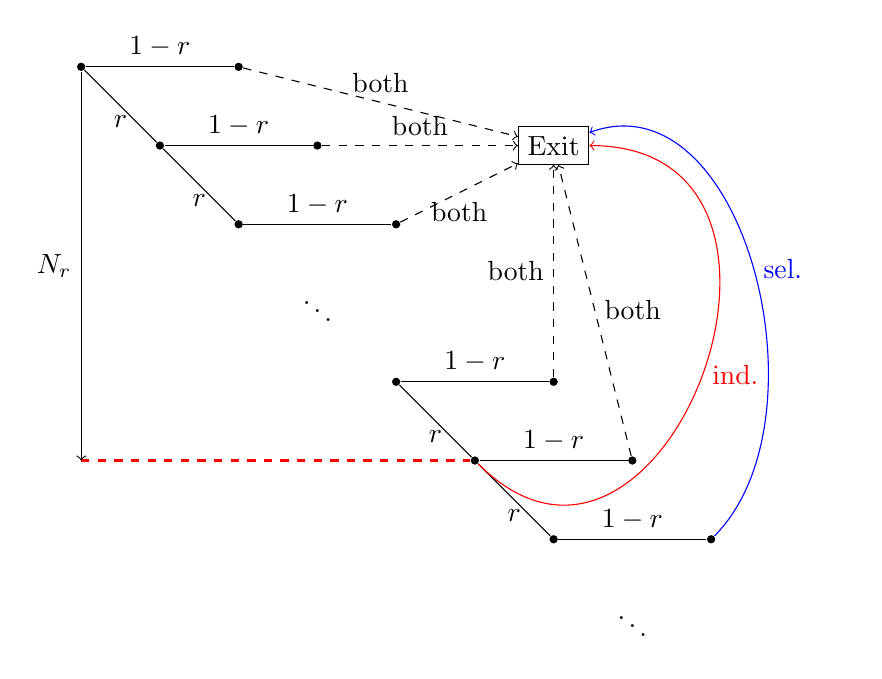
\begin{tikzpicture}
            \node [circle,fill=black,inner sep=0pt,minimum size=3pt]
                (1) at (0, 0) {};
            \node [circle,fill=black,inner sep=0pt,minimum size=3pt]
                (1full) at ($(1) + (2, 0)$) {};
            \node [circle,fill=black,inner sep=0pt,minimum size=3pt]
                (2) at (1, -1) {};
            \node [circle,fill=black,inner sep=0pt,minimum size=3pt]
                (2full) at ($(2) + (2, 0)$) {};
            \node [circle,fill=black,inner sep=0pt,minimum size=3pt]
                (3) at (2, -2) {};
            \node [circle,fill=black,inner sep=0pt,minimum size=3pt]
                (3full) at ($(3) + (2, 0)$) {};
            \node (etc) at (3, -3) {\(\ddots\)};
            \node [circle,fill=black,inner sep=0pt,minimum size=3pt]
                (N-1) at (4, -4) {};
            \node [circle,fill=black,inner sep=0pt,minimum size=3pt]
                (N-1full) at ($(N-1) + (2, 0)$) {};
            \node [circle,fill=black,inner sep=0pt,minimum size=3pt]
                (N) at (5, -5) {};
            \node [circle,fill=black,inner sep=0pt,minimum size=3pt]
                (Nfull) at ($(N) + (2, 0)$) {};
            \node [circle,fill=black,inner sep=0pt,minimum size=3pt]
                (N+1) at (6, -6) {};
            \node [circle,fill=black,inner sep=0pt,minimum size=3pt]
                (N+1full) at ($(N+1) + (2, 0)$) {};
            \node (etc2) at (7, -7) {\(\ddots\)};

            \draw (1) -- node [below] {\(r\)} (2);
            \draw (1) -- node [above] {\(1 - r\)} (1full);
            \draw (2) -- node [below] {\(r\)} (3);
            \draw (2) -- node [above] {\(1 - r\)} (2full);
            \draw (3) -- node [above] {\(1 - r\)} (3full);
            \draw (N-1) -- node [below] {\(r\)} (N);
            \draw (N-1) --  node [above] {\(1 - r\)} (N-1full);
            \draw (N) -- node [below] {\(r\)} (N+1);
            \draw (N) --  node [above] {\(1 - r\)} (Nfull);
            \draw (N+1) --  node [above] {\(1 - r\)} (N+1full);

            \node [draw] (exit) at (6, -1) {Exit};
            \draw [dashed, ->] (1full) -- node [above] {both} (exit);
            \draw [dashed, ->] (2full) -- node [above] {both} (exit);
            \draw [dashed, ->] (3full) -- node [below] {both} (exit);
            \draw [dashed, ->] (N-1full) -- node [left] {both} (exit);
            \draw [dashed, ->] (Nfull) -- node [right] {both} (exit);
            \draw [blue, ->] (N+1full) edge [out=45, in=20] node [right] {sel.} (exit);

            \draw [red, dashed, very thick] ($(N) - (5, 0)$) -- (N);
            \draw [->] (1) -- node [left] {\(N_r\)} (0, -5);
            \draw [red, ->] (N) edge[out=-45, in=0, looseness=2] node [right] {ind.}
                (exit);
        \end{tikzpicture}
    \end{center}
    \caption{Illustrative random walk showing the points at which an
    indiscriminate or a selective poacher will leave the park}

    \label{fig:random_walk}
\end{figure}

Using this, the expected time spent in the park \(T_1, T_2\) by poachers of both
types can be obtained:

For selective poachers:

\begin{align}
    T_1 &= (1-r)t + r(1-r)(1+t) + r^2(1-r)(2+t) + \dots\\
        &= (1-r)\sum_{i=0}^{\infty}r^i(i+t)\\
        &= (1-r)\left(1/r\sum_{i=0}^{\infty}ir^{(i+1)} + t\sum_{i=0}^{\infty}r^i\right)\\
        &= (1-r)\left(\frac{r}{(1-r)^2} + \frac{t}{1-r}\right) && \text{ using standard
formulae for geometric series}\\
    &= \frac{r+t(1-r)}{1-r}
\end{align}

For indiscriminate poachers:

\begin{align}
    T_2 &= (1-r)t + r(1-r)2t + r^2(1-r)3t + \dots + r^{N_r - 2}(1-r)(N_r - 1)t + r^{N_r - 1}N_rt\\
        &= (1-r)t\sum_{i=1}^{N_r - 1}ir^{i-1} + r^{N_r - 1}N_rt \\
        &= (1-r)t\left(\frac{1}{r \left(r - 1\right)^{2}} \left(N_{r} r
r^{N_{r}} - N_{r} r^{N_{r}} - r r^{N_{r}} + r\right)\right) + r^{N_r - 1}N_rt && \text{ using standard
formulae for geometric series}\\
        &= \frac{t}{r (1 - r)} \left(r^{2} + r^{N_{r}} - 2 r^{N_{r} + 1}\right)
\end{align}

Additionally, the poachers are also exposed to a risk. The risk to the poacher is
directly related to the proportion of rhinos not devalued, \(1 - r\), since
the rhino manager can spend more on security if the cost of devaluing is low.
In real life this is not always the case. The cost of security can be extremely
high thus it cannot be guaranteed that much security will be added from the
saved money. However, our model assumes that there is a proportional and negative
relationship between the measures.

\begin{eqnarray}
    \label{eqn:risk}
    (1 - r)^{\beta},
\end{eqnarray}

where \(\beta \geq 0\) is a constant that determines the precise relationship between
the proportion of rhinos not devalued and the security on the grounds. Therefore,
at any given time the expected cost for a poacher is,

\begin{eqnarray}
    \label{eqn:individual_cost}
        FT_i(1 - r)^{\beta} \text{ for } i \in \{1, 2\}
\end{eqnarray}
where \(F\) is a constants that determines the precise relationship. Fig.
\ref{fig:CostCurves} verifies the decreasing relationship between \(r\) and the
cost.

\begin{figure}[!htbp]
\begin{center}
    \begin{subfigure}{0.40\textwidth}
        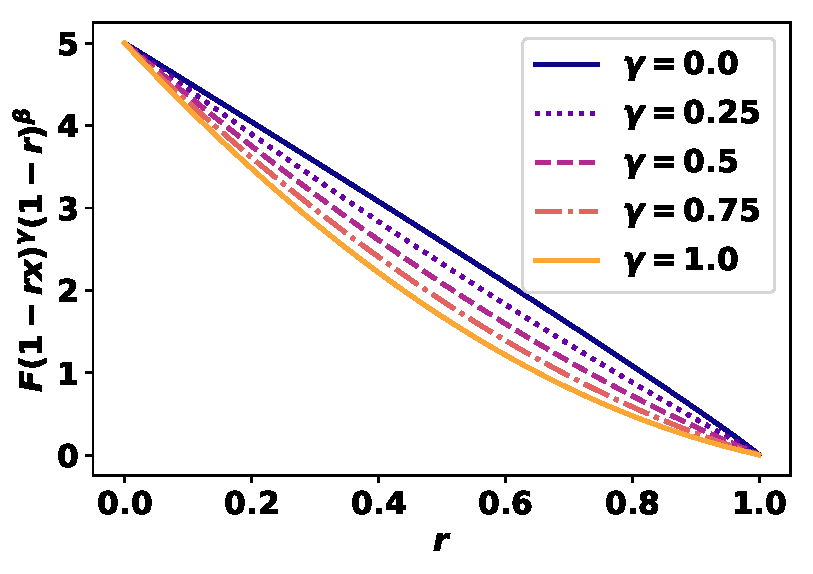
\includegraphics[width=\linewidth]{images/gammas_curve.pdf}
        \caption{For values, \(x=0.7, F=5\) and \(\beta=0.95\).}
    \end{subfigure}
    \begin{subfigure}{0.40\textwidth}
        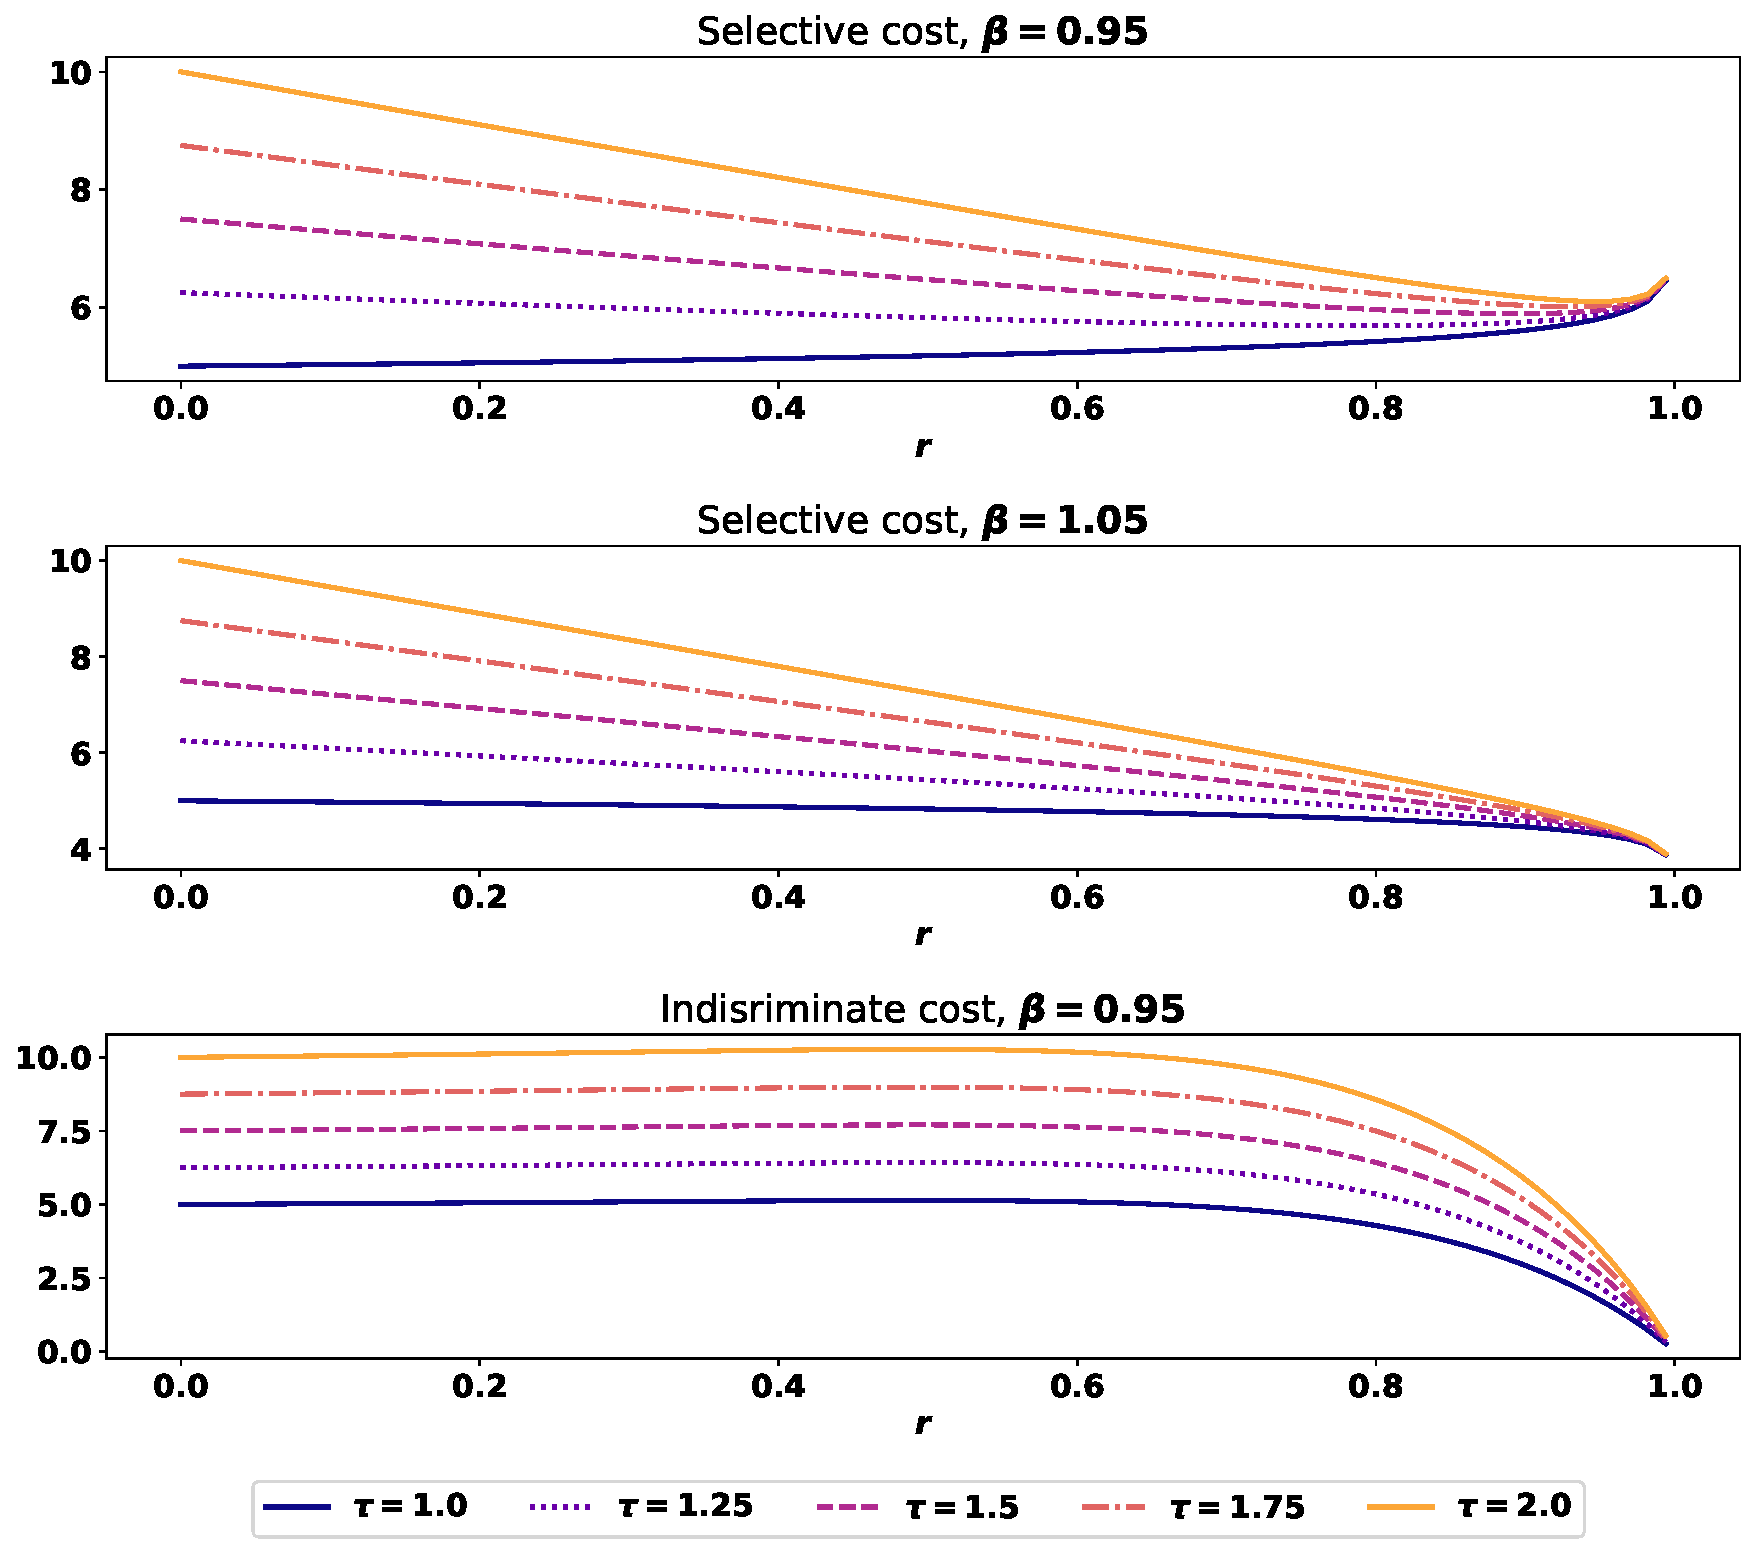
\includegraphics[width=\linewidth]{images/betas_curve.pdf}
        \caption{For values, \(x=1, F=5\) and \(\gamma=0.95\).}
    \end{subfigure}
\caption{\(F (1 - rx)^{\gamma} (1 - r)^{\beta}\).}\label{fig:CostCurves}
\end{center}
\end{figure}


To summarise, the cost incurred by a given individual poacher when interacting
with the population \(x\) is given by

\begin{eqnarray}
    \label{eqn:cost}
    \left\{
    \begin{array}{cl}
    \frac{1}{1 - r}  F\psi(r, x)^{\gamma} (1-r)^{\beta}& \mbox{ selective poacher}
    \\
    F\psi(r, x)^{\gamma} (1-r)^{\beta}& \mbox{ indiscriminate poacher.}
    \end{array} \right.
\end{eqnarray}

\noindent Combining~(\ref{eqn:gain}) and (\ref{eqn:cost}) gives the utility functions for
selective poachers, \(u_1(x)\), and indiscriminate poachers, \(u_2(x)\),

\begin{eqnarray}
\label{eqn:USchi}
u_1(x) &=& \theta(r,1) H \theta(r,x)^{-\alpha}
- \frac{1}{1- r} F\psi(r, x)^{\gamma} (1-r)^{\beta} ,
\\
\label{eqn:UnotSchi}
u_2(x) &=& \theta(r,0) H \theta(r,x)^{-\alpha}
- F\psi(r, x)^{\gamma}  (1-r)^{\beta}.
\end{eqnarray}


Let \(\sigma=(s, 1 - s)\) denote an individual where \(\sigma =(1, 0)\) represents
a selective poacher, and \(\sigma=(0, 1)\) represents an indiscriminate poacher.
For simplicity, from herein the individual \(\sigma\) is referred to in terms
of the probability of behaving selectively, \(\sigma=s\).
Thus the general utility function for an individual poacher in the population with
a proportion of \(0 \leq x \leq 1\) selective poachers is

\begin{eqnarray}
\label{eqn:utility}
u(s, x) = s u_1(x) +(1 - s) u_2(x).
\end{eqnarray}
Substituting~(\ref{eqn:USchi}) and~(\ref{eqn:UnotSchi}) into~(\ref{eqn:utility})
and using (\ref{eqn:theta}) and (\ref{eqn:psi}) gives,

\begin{eqnarray}
\label{eqn:tutility2}
u(s, x) &=&
H (\theta_r r(1-s) - r + 1)\theta(r,x)^{-\alpha} - F\left(1-s + \frac{s}{1-r} \right)(1-rx)^{\gamma}(1-r)^{\beta} .
\end{eqnarray}

In Section~\ref{section:evolutionary_stability}, the notions of stability
and evolutionary stability of these two strategies, as well as a potential
mixed strategy will be investigated.

%=======================================================
\section{Evolutionary Stability}\label{section:evolutionary_stability}

By definition, for a strategy to be an ESS it must first be a best response to an
environment where the entire population is playing the same strategy.
In our model there are three possible stable distributions based on the
equilibria of equation (\ref{eqn:u_differential_simplified}):

\begin{itemize}
    \item all poachers are selective;
    \item all poachers are indiscriminate;
    \item mixed population of selective and indiscriminate poachers.
\end{itemize}

\noindent Each of the equilibria will be examined in the following subsections.

\subsection{All poachers are selective}

\begin{theorem}\label{theorem:selective}
Using the utility model described in Section~\ref{section:the_model},
a population of selective poachers is unstable.
\end{theorem}

\begin{proof}
    For \(s=1\) to be a best response to itself the utility of behaving
    selectively in a population of selective poachers must be greater than the utility
    of a poacher behaving indiscriminately in a population of selective poachers,

    \begin{equation}
    u(1,1) > u(0,1),
    \end{equation}
    where

    \begin{eqnarray}
    \label{eqn:s1x1}
    u(1, 1) & = & H(1 -r)\theta(r, 1) ^ {- \alpha} - F (\frac{1}{1 - r})(1 - r)^{\gamma}(1 - r)^{\beta} \\
    & = & H(1 - r)^{1 - \alpha} - F(1 - r)^{\beta + \gamma - 1},
    \end{eqnarray}
    and

    \begin{eqnarray}
    \label{eqn:s0x1}
    u(0,1) & = & H(\theta_r r - r + 1)\theta(r, 1) ^ {- \alpha} - F (1 - r)^{\gamma}(1 - r)^{\beta} \\
           & = & H(\theta_r r +1 - r)(1 - r)^{-\alpha} - F(1 - r)^{\beta + \gamma}.
    \end{eqnarray}

    \noindent Setting~(\ref{eqn:s1x1}) to be greater than (\ref{eqn:s0x1}) gives the
    condition,
    \begin{eqnarray}
    \label{eqn:s1x1_s0x1}
    &&H \theta_r< -F(1 - r)^{\gamma + \beta + \alpha - 1}.
    \end{eqnarray}

    The right-hand side  will always be negative
    for any \(r\), on the other hand the left-hand side is always positive.
    Thus, (\ref{eqn:s1x1_s0x1}) can never hold.
\end{proof}

This implies that whilst~\cite{Lee} identified the individual poachers
acting selectively as an equilibrium it is an extremely weak equilibrium from
the point of view of population stability: a slight change and the population
will change.

\subsection{All poachers are indiscriminate}

\begin{theorem}\label{theorem:indiscriminate}
Using the utility model described in Section~\ref{section:the_model}, a population
of indiscriminate poachers is evolutionarily stable.
\end{theorem}

\begin{proof}
    In order for \(s=0\) to be an ESS it must
    remain the best response in a mutated population \(\chi_\epsilon\),
    where \(\chi_{\epsilon}=(x_\epsilon, 1 - x_\epsilon)\). Following the same
    notation, the mutated population will be denoted as \(x_\epsilon\) from
    herein. Thus,

    \begin{equation}\label{eqn:evolutionary_stability}
        u(0, x_\epsilon) > u(x_\epsilon, x_\epsilon),
    \end{equation}
    must hold. From (\ref{eqn:tutility2}),

    \begin{eqnarray}
        \label{eqn:u_indiscriminate_ess}
        u(0, x_\epsilon)  &=& H(\theta_rr - r + 1)\theta(r, x_\epsilon) ^{-\alpha}
        - F(1 - rx_\epsilon) ^ {\gamma} (1- r) ^ {\beta},
        \\
        \label{eqn:u_mutated_ess}
         u(x_\epsilon, x_\epsilon) &=& H(\theta_rr(1 - x_\epsilon)-r+ 1)\theta(r,
        x_\epsilon) ^{-\alpha} - F(1 - rx_\epsilon) ^ {\gamma} (1- r) ^
        {\beta}\left(1 -
        x_\epsilon + \frac{x_\epsilon}{1- r}\right).
\end{eqnarray}

    \noindent Let the difference of (\ref{eqn:u_indiscriminate_ess}) and (\ref{eqn:u_mutated_ess})
    be denoted as,

    \begin{eqnarray}
        \label{eqn:delta}
        \delta &=& u(0, x_\epsilon) - u(x_\epsilon, x_\epsilon),
          \\
         &=& H\theta(r,  x_\epsilon) ^{-\alpha} \theta_r r x_\epsilon -
        F(1 - r x_\epsilon) ^ {\gamma} (1- r) ^
        {\beta}x_\epsilon\left(\frac{-r}{1- r}\right).
    \end{eqnarray}
    All players being indiscriminate will be an ESS only if \(\delta >0 \) for any small
    value of \(\epsilon\). Thus only if,

    \begin{equation}
    \label{eqn:ess_inequality}
        H\theta(r, x_\epsilon) ^{-\alpha} \theta_r r x_\epsilon > F
        (1 - r x_\epsilon) ^ {\gamma} (1- r) ^ {\beta}
        x_\epsilon\left(\frac{-r}{1- r}\right).
    \end{equation}

    \noindent The right-hand side of inequality (\ref{eqn:ess_inequality}) is always negative
    since \((\frac{-r}{1- r}) < 0\)  for all \(r\). On the contrary, the left-hand
    side is always positive for all \(r\), thus the inequality always holds.
    Therefore, it is proven that all indiscriminate poachers is an evolutionary
    stable strategy.
\end{proof}

This shows that a population of indiscriminate poachers
not only corresponds to the equilibrium of the individual based
game identified in~\cite{Lee}, but is also a very robust and attractive
equilibrium at the population level.

\subsection{Mixed population of selective and indiscriminate poachers}

\begin{theorem}\label{theorem:mixed}
Using the utility model described in section~\ref{section:the_model}, a mixed
stable population (\(s=s^*\)) never exists for \(0 < r <1\).
\end{theorem}

\begin{proof}
    A mixed strategy \(s = s^*\) is said to be stable for a
    given \(s^*\) only if,

    \begin{eqnarray}
    \label{eqn:s1xs_s0xs}
    u(1,s^*) = u(0,s^*).
    \end{eqnarray}
    From equation (\ref{eqn:tutility2}) the left-hand side is,

    \begin{eqnarray}
    \label{eqn:mixed_lhs}
    u(1,s^*)&=&
    H(1 - r) \theta(r, s^*)^{-\alpha} - F \frac{1}{(1 - r)}(1 - rs^*)^{\gamma}(1 - r)^{\beta}
    \end{eqnarray}
    and the right-hand side is

    \begin{eqnarray}
    \label{eqn:mixed_rhs}
    u(0,s^*)&=&
    H(\theta_rr + 1 - r)\theta(r, s^*)^{-\alpha} - F(1 - rs^*)^{\gamma}(1 - r)^{\beta}.
    \end{eqnarray}
    Substituting (\ref{eqn:mixed_lhs}) and (\ref{eqn:mixed_rhs}) into~(\ref{eqn:s1xs_s0xs}) gives

    \begin{eqnarray}\label{eqn:stable_mixed}
        u(1,s^*) - u(0,s^*) & = & H\theta(r, s^*)^{-\alpha} (-\theta_r r)  + F (1 - rs^*)^{\gamma}(1 - r)^{\beta}(\frac{r}{1-r})\\
    \label{eqn:stable_mixed_condition}
      & = &   - r (H \theta_r \theta(r, s^*)^{-\alpha}  + F (1 - rs^*)^{\gamma}(1 - r)^{\beta - 1}) = 0.
    \end{eqnarray}
    Condition~(\ref{eqn:stable_mixed_condition}) can never hold for \(0 < r <1\)
    because both terms of the sum are positive. Thus a mixed stable equilibrium
    is never stable.
\end{proof}

In this section we have analytically studied the stability of all the possible
equilibria. We have proven the instability of any population with selective
poachers,
and the evolutionary stability of the indiscriminate behaviour.
All of these theoretic results have been verified empirically, and the data for this
has been archived at~\cite{Glynatsi2017}.

Theorems~\ref{theorem:selective},~\ref{theorem:indiscriminate},~\ref{theorem:mixed}
are illustrated in Fig.~\ref{fig:indiscriminate_ess}
which shows the numerical solutions to (\ref{eqn:u_differential_simplified})
using (\ref{eqn:USchi}) and  (\ref{eqn:UnotSchi}) with \(x_1=x\).
This is done using numerical integration implemented  in~\cite{scipy}.
As evidenced from the scenarios considered, all populations converge
to being all indiscriminate.

\begin{figure}[!htbp]
    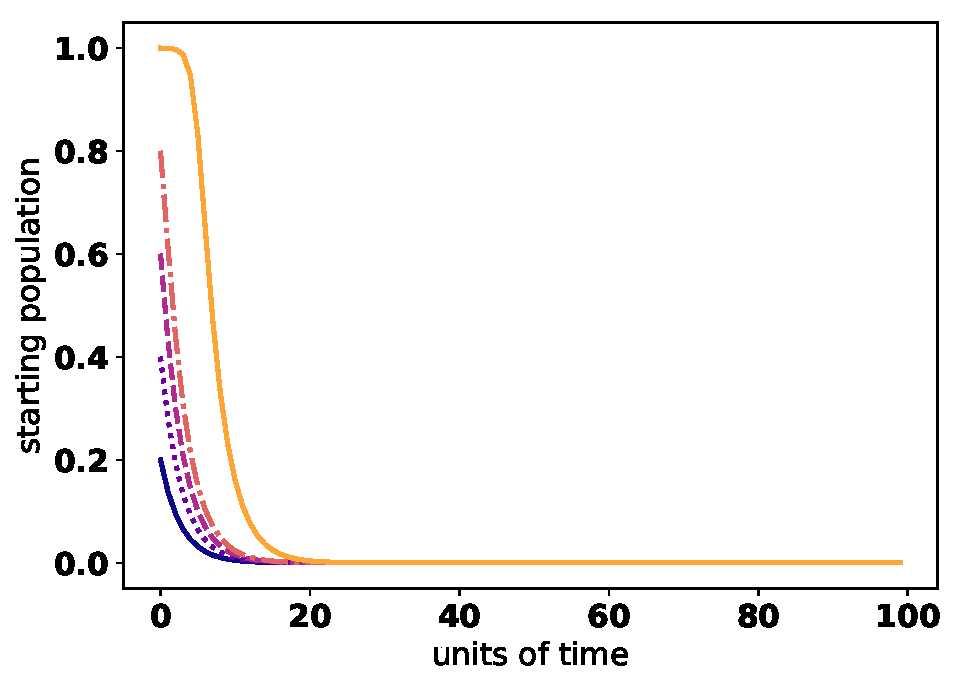
\includegraphics[width=\textwidth]{images/IndiscriminateESS.pdf}
    \caption{\label{fig:indiscriminate_ess} The change of the population over
    time with different starting populations. For \(F=5, H=50,
    \alpha=2, \beta=2, \gamma=1, \theta_r=0.6\).}
\end{figure}

Note that these results essentially follow by comparing equations (\ref{eqn:USchi})
and (\ref{eqn:UnotSchi}), which show that \(u_1(x) \leq u_2(x)\) for all \(x\).
Consider the reverse scenario,

\begin{align}
    u_1(x) & > u_2(x)\\ 
    F\psi(r, x) ^ {\gamma} (1 - r) ^ {\beta - 1} & < -H \theta(r, x) ^ {-\alpha} \theta_r
\end{align}

\noindent which gives the required contradiction. This shows that the utility model used
implies that given the choice of acting selectively or indiscriminately, in any
given environment, it will always be a rational deviation to act
indiscriminately.

In the following section a disincentive to acting indiscriminately will be
introduced. This can be interpreted in many ways:

\begin{itemize}
    \item more severe punishment for indiscriminate killing of rhinos;
    \item educational interventions that highlight the negative aspects of
        indiscriminate killing;
    \item the possibility of a better alternative being offered to selective
        poachers.
\end{itemize}

\section{Disincentive for indiscriminate behaviour}

Let us consider the following modification of the utility to an indiscriminate
poacher:

\begin{equation}
    \label{eqn:modified_utility_for_ind}
    \tilde u_2(x) = u_2(x) - \Gamma
\end{equation}
where \(\Gamma>0\) is some constant representing a disincentive only applied to
indiscriminate poachers. This leads to the following modified form of (\ref{eqn:utility}):

\begin{equation}
    \label{eqn:modified_utility}
    \tilde u(s, x) = u(s, x) - (1 - s) \Gamma.
\end{equation}

\noindent This leads to the following theorem:

\begin{theorem}\label{theorem:selective_new_utility}
Using the modified utility model described
a population of selective poachers is stable if and only if:

\begin{equation}\label{eq:selective_condition_new_utility}
\theta_r H -  F(1 -r) ^{\gamma + \beta + \alpha -1} < \frac{\Gamma (1- r) ^ {\alpha}}{r}.
\end{equation}

\end{theorem}

\begin{proof}
    Following a similar structure to that of Theorem~\ref{theorem:selective},

    \begin{equation}
    \tilde{u}(1,1) > \tilde{u}(0,1),
    \end{equation}
    where

    \begin{eqnarray}
    \label{eqn:s1x1_new_utility}
    \tilde{u}(1,1) = H(1 - r)^{1 - \alpha} - F(1 - r)^{\beta + \gamma - 1},
    \end{eqnarray}
    and

    \begin{eqnarray}
    \label{eqn:s0x1_new_utility}
    \tilde{u}(0,1) = H(\theta_r r +1 - r)(1 - r)^{-\alpha} - F(1 - r)^{\beta + \gamma} - \Gamma.
    \end{eqnarray}

    \noindent Setting~(\ref{eqn:s1x1_new_utility}) to be greater than (\ref{eqn:s0x1_new_utility})
    gives the condition,

    \begin{eqnarray}
    \label{eqn:s1x1_s0x1_new_utility}
    &&\theta_r H -  F(1 -r) ^{\gamma + \beta + \alpha -1} < \frac{\Gamma (1- r) ^ {\alpha}}{r}.
    \end{eqnarray}
\end{proof}

\noindent This immediately leads to the following important remark:

\begin{theorem}\label{theorem:devaluating_rhinos}
Using the modified utility model described,
if all rhinos have been dehorned a population of selective poachers is not
stable.
\end{theorem}

\begin{proof}
All rhinos being dehorned implies that \(r=1\). Substituting this into
(\ref{eq:selective_condition_new_utility}) gives,

\begin{equation}
    \theta_r H < 0,
\end{equation}
which is not possible.
\end{proof}

Theorem~\ref{theorem:devaluating_rhinos} is due to the fact that given two
options, if all rhinos have been dehorned then all poachers will need to act
indiscriminately to have any source of utility. Theorem~\ref{theorem:selective_new_utility}
states that a  mixed population can be stable with a disincentive, as opposed to
Theorem~\ref{theorem:mixed} which states that a mixed stable strategy does not
exist for \(0 <r <1\). This is illustrated in Fig.~\ref{fig:ess-new-utility} where
the evolutionary dynamics are represented for a number of scenarios.

Note that now the manager has control over the point of convergence by
controlling \(r\), as shown in Fig.~\ref{fig:convergence-over-r}
where
a difference in the value from \(r=0.7\) to \(r=0.5\) changes the point of
convergence from a mixed to a selective one. Moreover, the manager can also
manipulate how fast the population convergences, as shown in the difference from
\(r=0.5\) to \(r=0.2\). Fig~\ref{fig:equilibrium-over-r-tilde-u} shows the
equilibrium for \(x\) for a number of different values of \(r\), and indicates
that having a large \(r\) pushes poachers to behave indiscriminately. However all
selective poachers can save at most, the $r$ proportion of dehorned rhinos, so a
low \(r\) is not ideal. As demonstrated in Fig~\ref{fig:equilibrium-over-H-tilde-u},
a higher value of \(H\) also has a non-ideal effect on the poachers, as one would
expect. Thus, high values of \(H\) and \(r\) lead to more indiscriminate poachers.

\noindent The insights gained from the results are discussed in Section~\ref{section:discussion}.

\begin{figure}[!htbp]
    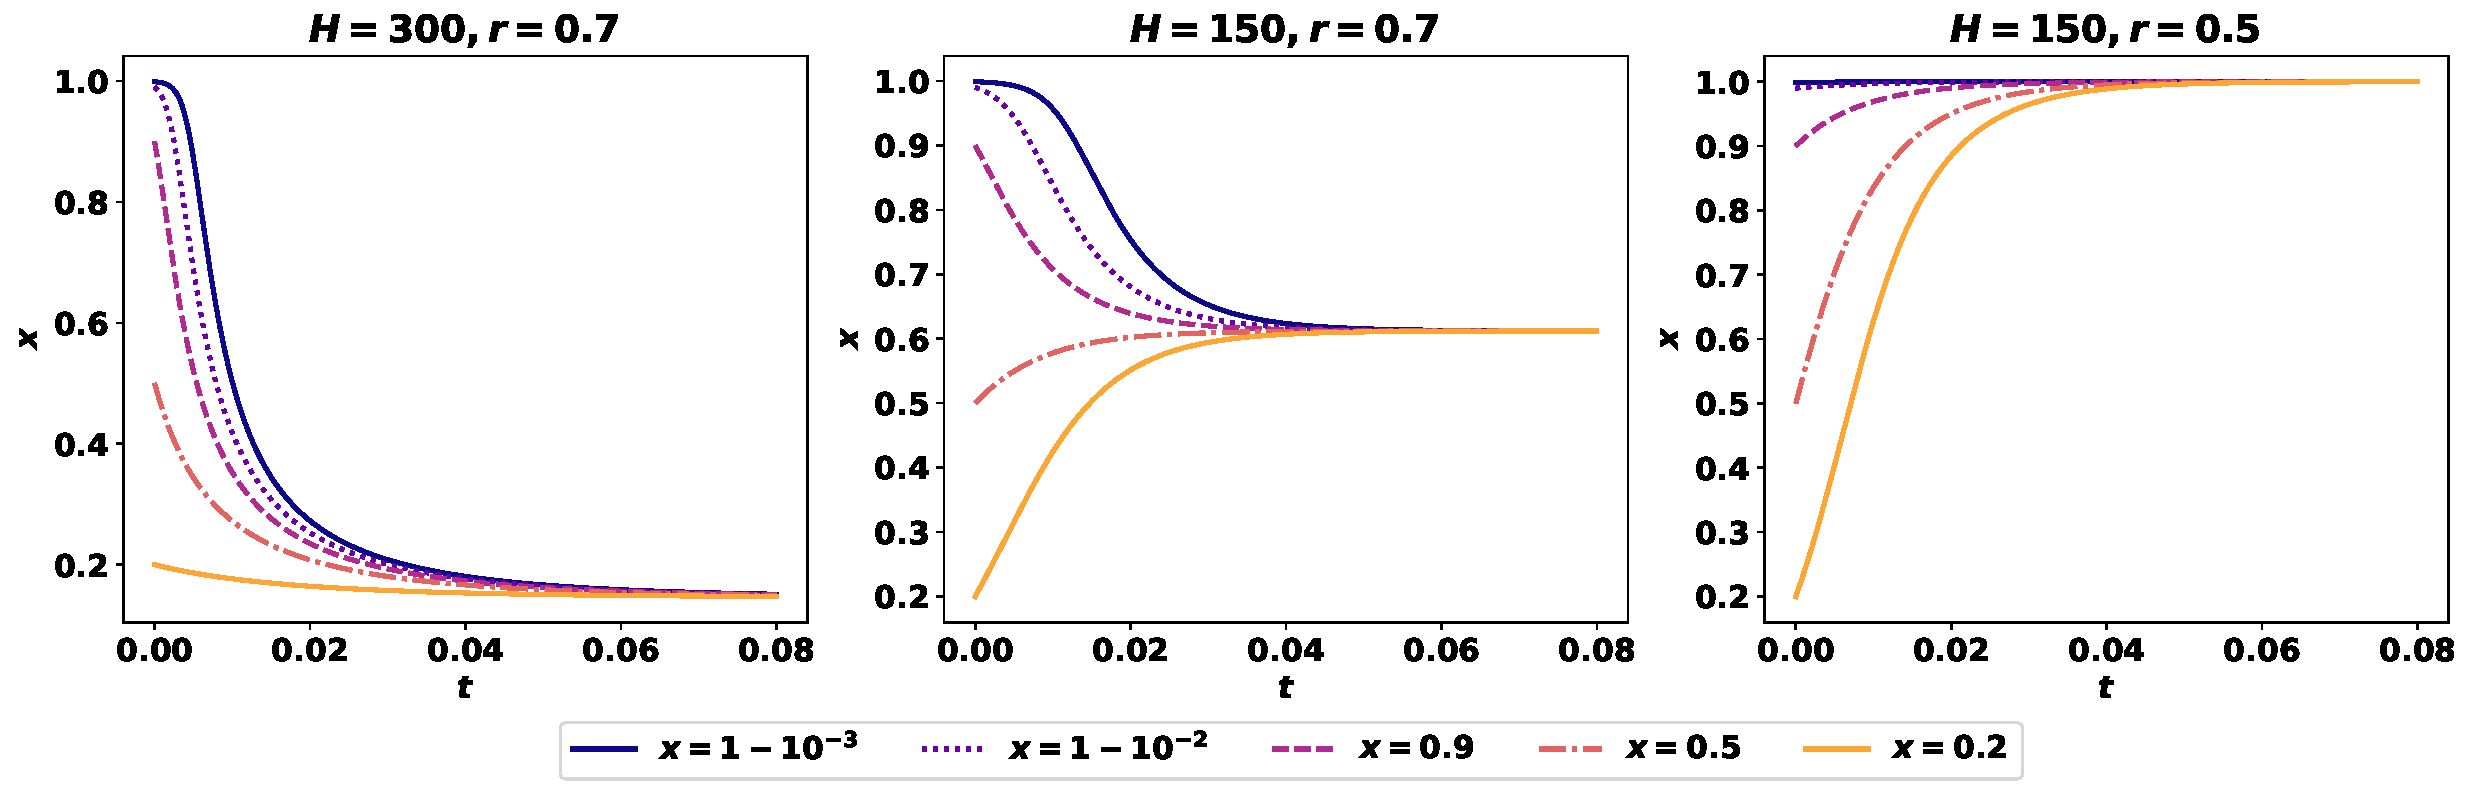
\includegraphics[width=\textwidth]{images/ESS-new-utility.pdf}
    \caption{The change of the population over
    time with different starting populations with a disincentive. For \(F=50, \alpha=2,
    \beta=2, \gamma=1, \theta_r=0.5, \Gamma=300\).}
    \label{fig:ess-new-utility}
\end{figure}

\begin{figure}[!htbp]
    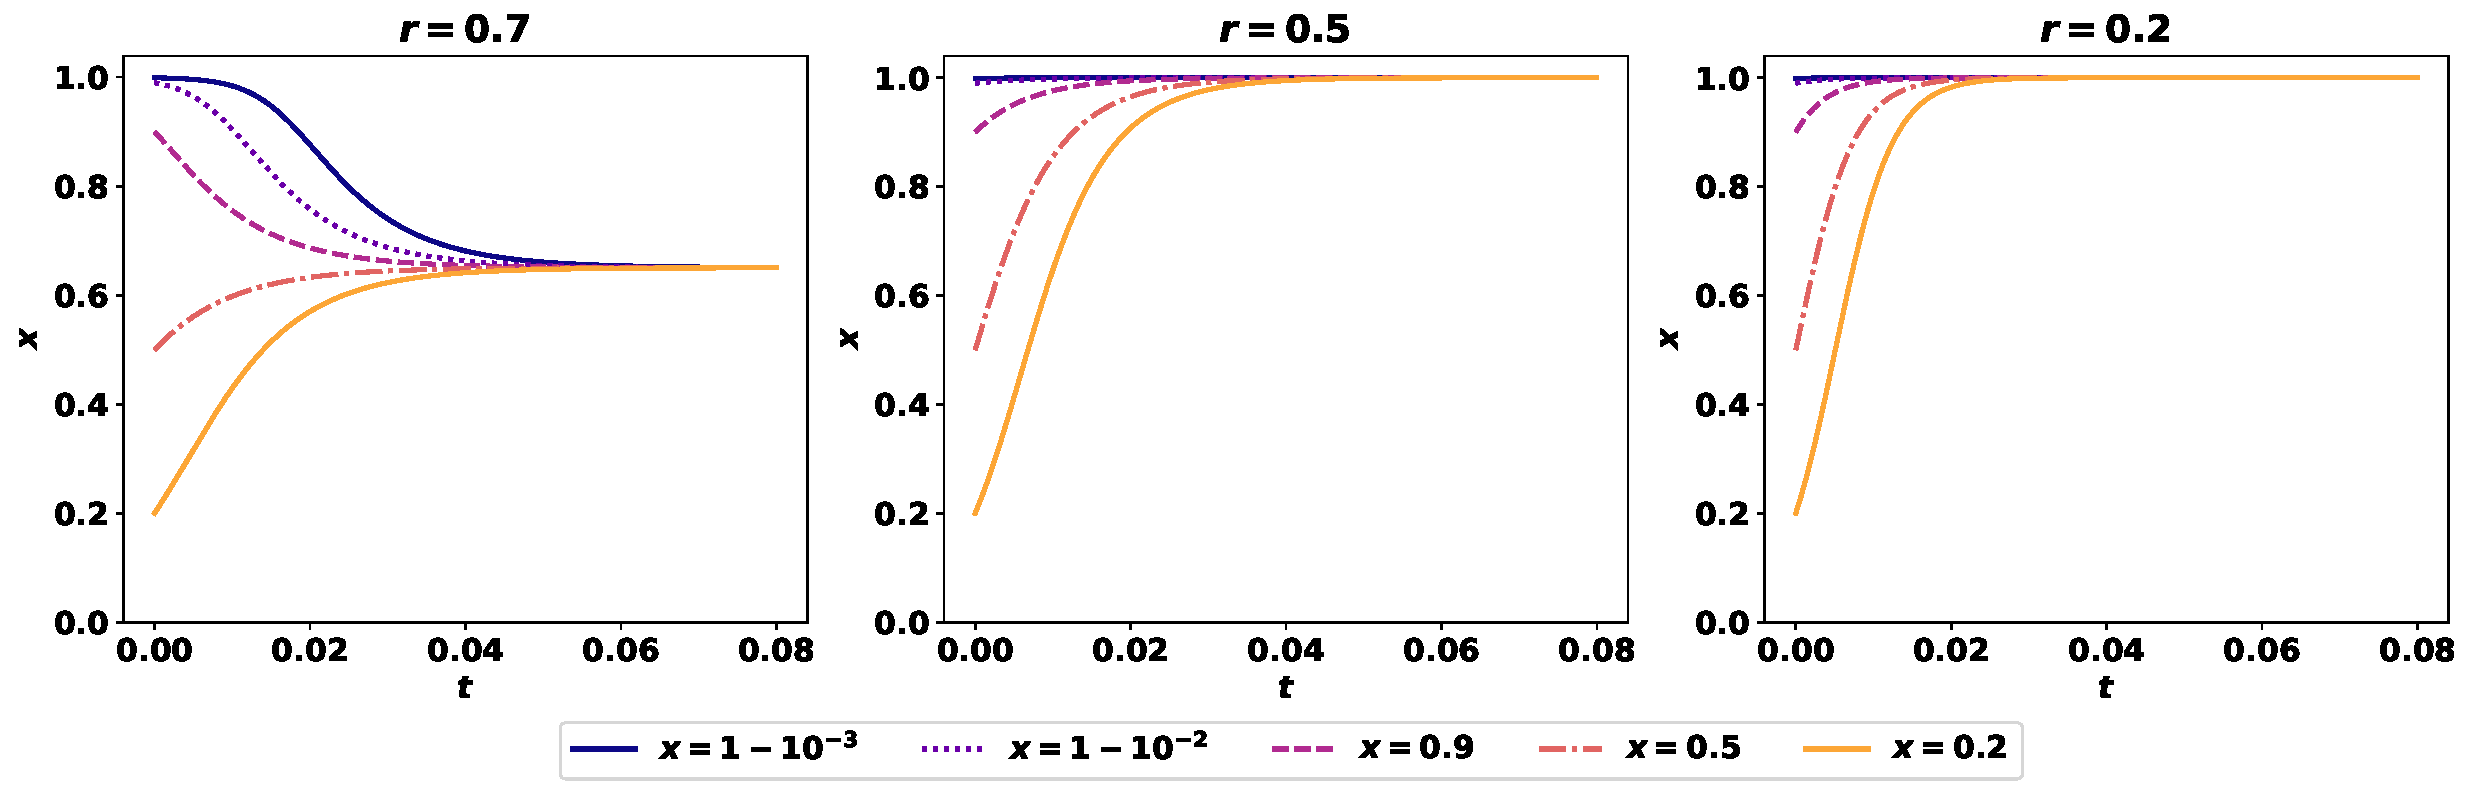
\includegraphics[width=\textwidth]{images/ESS-new-utility-based-r.pdf}
    \caption{The change of the convergence point with different values of \(r\)
    with different starting populations with a disincentive. For \(F=50, H=150,
    \alpha=2, \beta=2, \gamma=1, \theta_r=0.5, \Gamma=300\).}
    \label{fig:convergence-over-r}
\end{figure}

\begin{figure}[!htbp]
\centering
    \begin{subfigure}{.5\textwidth}
        \centering
        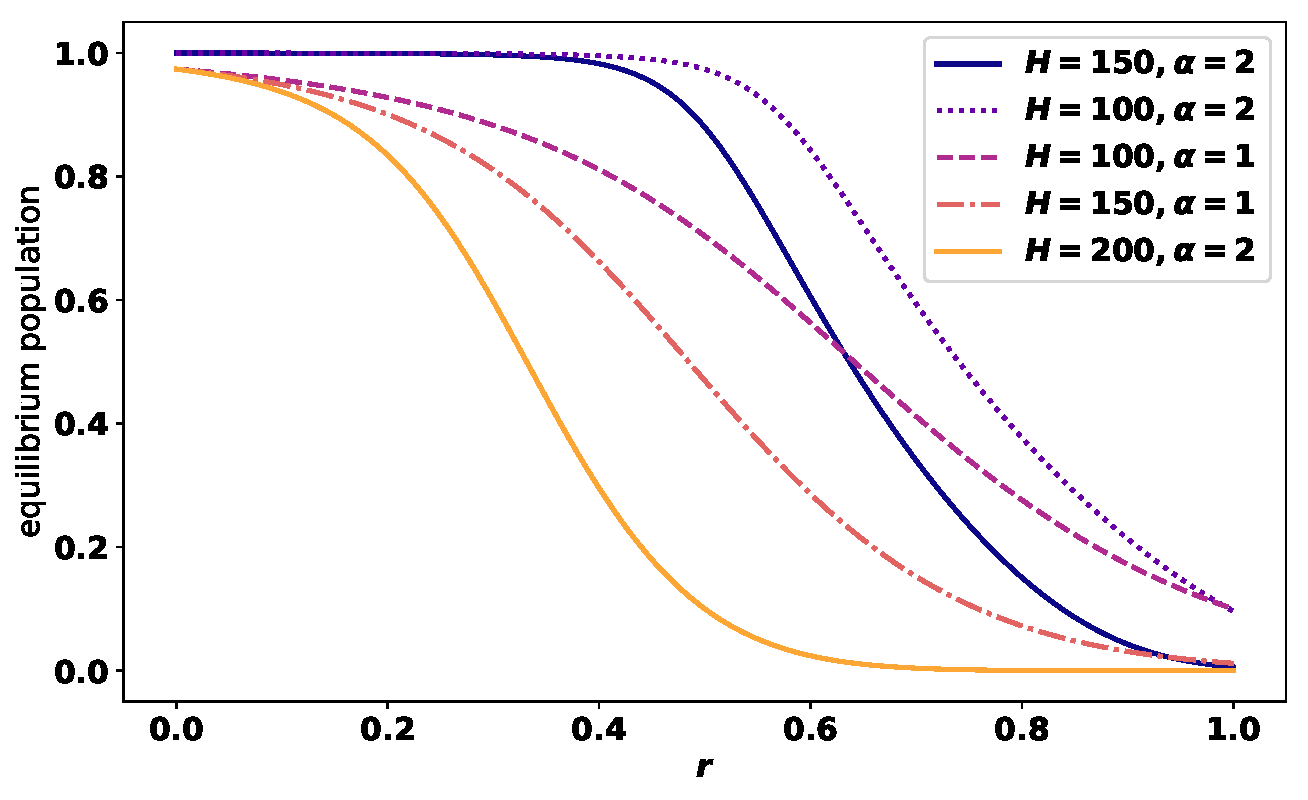
\includegraphics[width=0.95\textwidth]{images/new-utility-over_r.pdf}
        \caption{Effect of \(r\) for \(F=50, \beta=2, \gamma=1, \theta_r=0.6\).}
        \label{fig:equilibrium-over-r-tilde-u}
    \end{subfigure}
    ~
    \begin{subfigure}{.5\textwidth}
        \centering
        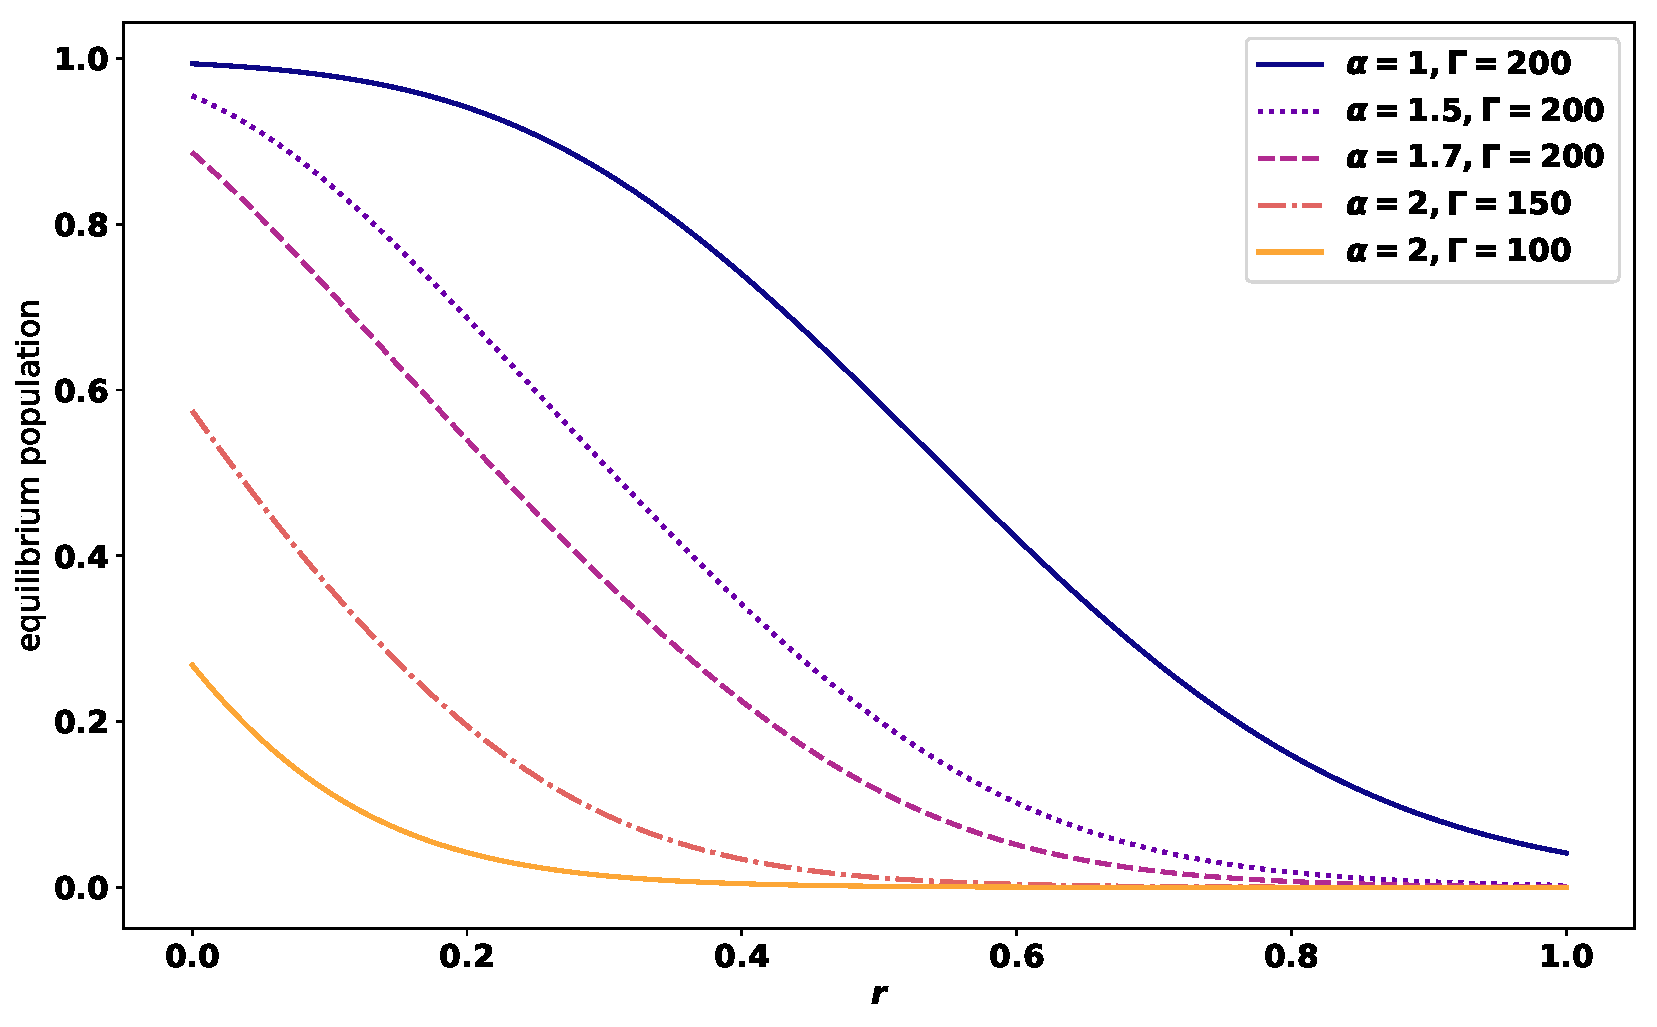
\includegraphics[width=0.95\textwidth]{images/new-utility-over_H.pdf}
        \caption{Effect of \(H\) for \(F=50, r=0.6, \beta=2, \gamma=1, \theta_r=0.6\).}
        \label{fig:equilibrium-over-H-tilde-u}
    \end{subfigure}
    \caption{Equilibrium behaviour with a disincentive.}
\end{figure}

%=============================================================
\section{Discussion and Conclusions}
\label{section:discussion}

In this work the dynamics of a selective population were explored. It was proven
that being selective is not a best response even in a population where
everyone is behaving selectively. More specifically, even a mixed population with
a small percentage of the population behaving selectively will not persist. Thus,
a poacher would never adopt a selective strategy over an indiscriminate one.

Using a realistic and generic utility model it was found that
the only strategy that was proven to be stable is the indiscriminate one.
Moreover, it was proven to be evolutionary stable as well. Meaning,
that for any given starting population, the poachers would evolve to adopt an
indiscriminate behaviour.

Our results indicate however that it is possible for a population of selective
poachers to exist, but for this to occur a disincentive must be applied to the
utility of indiscriminate poachers. Numerical results indicate that even in this
case, the more rhinos which are dehorned, the less probability that a poacher
will be selective. Assuming basic supply and demand arguments, the demand of
a partial horn will increase by removing horns thus the probability
of being selective decreases. Therefore, even in the scenario with a
disincentive, the proportion of rhinos which could be saved is limited, so
approaches which aim to reduce demand (as suggested in~\cite{Duan2013})
would have more potential.

The disincentive factor can have several interpretations. According to~\cite{Duan2017},
engaging the rural communities that neighbour or live with wildlife is the
key to fighting the illegal trade of wildlife. Strengthening disincentives for
illegal behaviour can be interpreted as the disincentive factor. Likewise,
increasing incentives for wildlife stewardship, decreasing the cost of living
with wildlife, and supporting livelihood that is not related to poaching can
serve as incentives for selective behaviour.

Note that the proportion of dehorned rhinos \(r\) is continuous over \([0, 1]\)
in the model. However, standard practice of a given park manager in almost all
cases is to either dehorn all the animals in a defined enclosed area, or none
at all. This is thought to be because partial dehorning tends to disturb
rhino social structures. The theoretic model presented here, whilst allowing for
consideration at the park level with park managers playing a mixed strategy, also
can be considered at the macroeconomic level. Where \(r\) represents the quantity
of dehorned rhinos available across multiple parks.

The insights gained, notably that a population of selective poachers is
sustainable only if a large disincentive is in place (even if all rhinos have
been dehorned) have implication at the long term national policy level.

Following discussions with environmental specialists it is clear that dehorning
is empirically thought to be one of the best responses to poaching. This
indicates that whilst of theoretic and macroeconomic interest, the modelling
approach investigated in this work has potential for further work. For example,
a detailed study of two neighbouring parks with differing policies could be
studied using a game theoretic model. Another interesting study would be to
introduce a third strategy available to poachers: this would represent the
possibility of not poaching (perhaps finding another source of income) and/or
leaving the current environment to poach elsewhere.

\section*{Authors' contributions}

All authors conceived the ideas and designed the methodology. NG and VK developed the
source code needed for the numerical experiments and generating the data. All authors
contributed critically to the drafts and gave final approval for publication.

\section*{Acknowledgements}

This work was performed using the computational facilities of the Advanced
Research Computing @ Cardiff (ARCCA) Division, Cardiff University.

A variety of software libraries have been used in this work:

\begin{itemize}
    \item The Scipy library for various algorithms~\cite{scipy}.
    \item The Matplotlib library for visualisation~\cite{hunter2007matplotlib}.
    \item The SymPy library for symbolic mathematics~\cite{sympy}.
    \item The Numpy library for data manipulation~\cite{walt2011numpy}.
\end{itemize}

Finally, we would like to express our appreciation to David Roberts and Michael 't
Sas-Rolfes for their valuable and constructive suggestions for this research.
We would also like to thank
Dr. Jonathan Gillard for his careful reading and double checking of the algebra in the paper.

\section*{Data Accessibility}

The data generated for this work have been archived and are available
online~\cite{Glynatsi2017}.

\bibliographystyle{plain}
\bibliography{bibliography.bib}

\end{document}
